\documentclass[frenchb, paper=a4, fontsize=11pt]{scrartcl}

\usepackage[utf8x]{inputenc}
\usepackage[T1]{fontenc}
\usepackage{lmodern}

\usepackage{url}

% Color
% cfr http://en.wikibooks.org/wiki/LaTeX/Colors
\usepackage{color}
\usepackage[usenames,dvipsnames,svgnames,table]{xcolor}
\definecolor{dkgreen}{rgb}{0.25,0.7,0.35}
\definecolor{dkred}{rgb}{0.7,0,0}

\newcommand{\matlab}{\textsc{Matlab}}

% Math symbols
\usepackage{amsmath}
\usepackage{amssymb}
\usepackage{amsthm}

\newcommand\eqdef{\triangleq}

\DeclareMathOperator{\newdiff}{d} % use \dif instead
\newcommand{\dif}{\newdiff\!}
\newcommand{\fpart}[2]{\frac{\partial #1}{\partial #2}}
\newcommand{\ffpart}[2]{\frac{\partial^2 #1}{\partial #2^2}}
\newcommand{\fdpart}[3]{\frac{\partial^2 #1}{\partial #2\partial #3}}
\newcommand{\fdif}[2]{\frac{\dif #1}{\dif #2}}
\newcommand{\ffdif}[2]{\frac{\dif^2 #1}{\dif #2^2}}
\newcommand{\constant}{\ensuremath{\mathrm{cst}}}

\usepackage{siunitx}

\usepackage{tikz}

\usepackage{lmodern}
%\usepackage[protrusion=true,expansion=true]{microtype}
\usepackage{xspace}

\usepackage{babel}

\KOMAoptions{DIV=last}

\usepackage{hyperref}
\usepackage{todonotes}
\DeclareSIUnit{\rot}{rot}
\usepackage[makeroom]{cancel}
\usepackage{todonotes}
\usepackage{epstopdf}

%%% Custom sectioning (sectsty package)
\usepackage{sectsty}								% Custom sectioning (see below)
\allsectionsfont{\scshape}						% Change font of al section commands

%%% Custom headers/footers (fancyhdr package)
\usepackage{fancyhdr}
\pagestyle{fancyplain}
\fancyhead{}										% No page header
\fancyfoot[L]{\small Groupe 1}					% You may remove/edit this line 
\fancyfoot[C]{}									% Empty
\fancyfoot[R]{\thepage}							% Pagenumbering
\renewcommand{\headrulewidth}{0pt}				% Remove header underlines
\renewcommand{\footrulewidth}{0pt}				% Remove footer underlines
\setlength{\headheight}{13.6pt}

%%% Equation and float numbering
\numberwithin{equation}{section}					% Equationnumbering: section.eq#
\numberwithin{figure}{section}					% Figurenumbering: section.fig#
\numberwithin{table}{section}						% Tablenumbering: section.tab#

%%% Maketitle metadata
\newcommand{\horrule}[1]{\rule{\linewidth}{#1}} 	% Horizontal rule

\title{
		%\vspace{-1in} 	
		\usefont{OT1}{bch}{b}{n}
		\normalfont \normalsize \textsc{Ecole polytechnique de Louvain} \\ [25pt]
		\horrule{0.5pt} \\[0.4cm]
		\large LINMA1510 - Automatique linéaire\\
		\huge Laboratoire 3 - Régulation de la tension aux bornes d'un circuit
		électrique à l'aide d'un régulateur industriel \\
		\horrule{1.5pt} \\[0.5cm]
}
\author{
		\normalfont
		\textsc{Groupe 62}\\
      	Antoine Paris\hspace{0.6cm} Philippe Verbist \\	
       	\normalsize
        \today
}
\date{}

\begin{document}
\maketitle

\section{Système linéarisé}
Le système linéarisé autour de $\bar{i}_{\%}=50\%$, $\bar{V}_1 = 4.9$
et $\bar{R}_p = R_1 = 0.47k\/Omega$
se  présente sous la forme
\begin{equation}
\left\{ \begin{array}{lcl}
\dot{x}_1 &=& -a_{11}x_1 + a_{12} x_2 + bu + dv\\
\dot{x}_2 &=& a_{21} x_1 -a_{22} x_2\\
y&=& 10x_2 \quad \text{ou } y=-10x_1 + 20x_2
\end{array}\right.
\end{equation}
avec 
\begin{equation}
\left\{\begin{array}{lclcl}
a_{11} &=& \frac{1}{C_1}(\frac{1}{\bar{R}_p} + \frac{1}{R_{12}}) &=& 1.06\\
a_{12} &=& \frac{1}{C_1 R_{12}} &=& 0.097\\
a_{21} &=& \frac{1}{C_1 R_{12}} &=& 0.097\\
a_{22} &=& \frac{1}{C_2R_{12}} &=& 0.097\\
b &=& \frac{1}{5C_1} &=& 0.091\\
d &=& \frac{\bar{V}_1}{C_1\bar{R}_p^2} &=& 9.67
\end{array}\right.
\end{equation}

On a également
\begin{align}
A &= \bigg[\begin{array}{cc}
-a_{11} & a_{12}\\
a_{21} & -a_{22}
\end{array} \bigg]\\
B_u &= \bigg[\begin{array}{c}
b\\
0
\end{array} \bigg], \quad
B_v = \bigg[\begin{array}{c}
d\\
0
\end{array} \bigg]\\
C &= \bigg[\begin{array}{c}
0\\
10
\end{array} \bigg]
\quad \text{ou } C =\bigg[\begin{array}{c}
-10\\
20
\end{array} \bigg]\\
D&=0
\end{align}

\section{Fonctions de transfert en boucle ouverte}
\paragraph{Minimum de phase}
Le système nous est donné:
\begin{align*}
\dot{x}_1 &= -a_{11}x_1 + a_{12}x_2 + bu + dv\\
\dot{x}_2 &= a_{21}x_1 - a_{22} x_2\\
y&= 10x_2
\end{align*}
On trouve rapidement les fonctions de transfert
\begin{align*}
G_A(s) &= C(sI-A)^{-1} B_u + D\\
&=\frac{10ba_{21}}{s^2 + (a_{11}+a_{22})s + a_{11}a_{22} - a_{12}a_{21}}\\
&=\frac{0.08792}{s^2+1.161s+0.09353}
= \frac{0.08792}{(s+1.073)(s+0.08714)}\\
H_A(s) &= C(sI-A)^{-1} B_v + D\\
&=\frac{10da_{21}}{s^2 + (a_{11}+a_{22})s + a_{11}a_{22} - a_{12}a_{21}}\\
&=\frac{9.751}{s^2+1.161s+0.09353}
= \frac{9.751}{(s+1.073)(s+0.08714)}
\end{align*}

\paragraph{Non-minimum de phase}

Le système est le même que précédemment, sauf que:
\begin{align*}
y&= -10x_1 + 20x_2
\end{align*}
On trouve rapidement les fonctions de transfert
\begin{align*}
G_B(s) &= \frac{-10 b (s-2a_{21}+a_{22})}{s^2 + (a_{11}+a_{22})s + a_{11}a_{22}-a_{12}a_{21}}\\
&=\frac{-0.9091s+0.08792}{s^2+1.161s+0.09353} = \frac{-0.90909(s-0.09671)}{(s+1.073)(s+0.08714)}\\
H_B(s) &= \frac{-10 d (s-2a_{21}+a_{22})}{s^2 + (a_{11}+a_{22})s + a_{11}a_{22}-a_{12}a_{21}}\\
&=\frac{-100.8s+9.751}{s^2+1.161s+0.09353}
=\frac{-100.83(s-0.09671)}{(s+1.073)(s+0.8714)}
\end{align*}

\section{Mesure des temps d'établissement}
Les réponses normalisées à la pertubation des deux systèmes sont
reprises sur la figure \ref{fig:settling-time}. Comme attendu,
les temps d'établissement sont identiques dans les deux cas
\begin{equation}
	t_R = \SI{45}{\second}.
\end{equation}

\begin{figure}[ht]
	\centering
	% This file was created by matlab2tikz.
%
%The latest updates can be retrieved from
%  http://www.mathworks.com/matlabcentral/fileexchange/22022-matlab2tikz-matlab2tikz
%where you can also make suggestions and rate matlab2tikz.
%
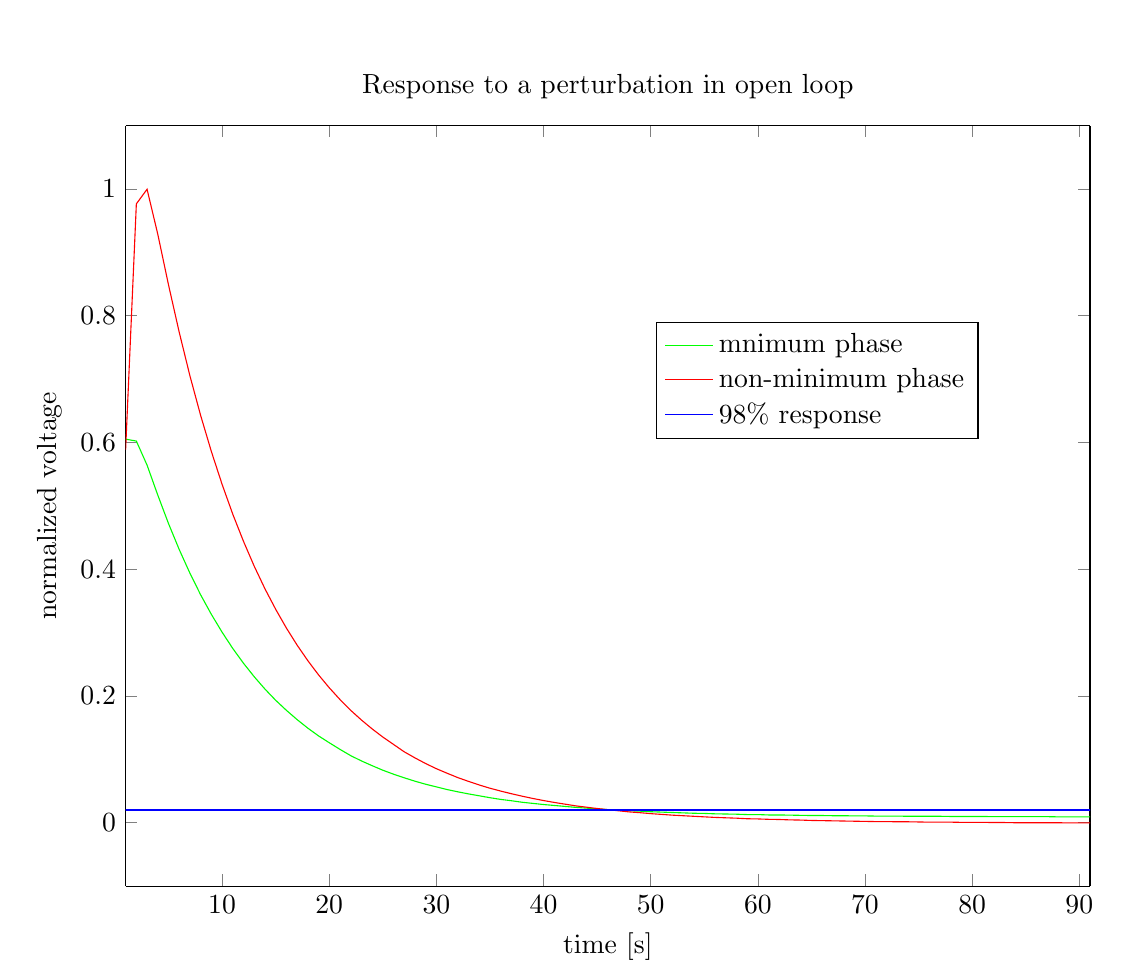
\begin{tikzpicture}

\begin{axis}[%
width=4.822in,
height=3.803in,
at={(0.809in,0.513in)},
scale only axis,
separate axis lines,
every outer x axis line/.append style={black},
every x tick label/.append style={font=\color{black}},
xmin=1,
xmax=91,
xlabel={time [s]},
every outer y axis line/.append style={black},
every y tick label/.append style={font=\color{black}},
ymin=-0.1,
ymax=1.1,
ylabel={normalized voltage},
axis background/.style={fill=white},
title={Response to a perturbation in open loop},
legend style={at={(0.55,0.588)},anchor=south west,legend cell align=left,align=left,draw=black}
]
\addplot [color=green,solid]
  table[row sep=crcr]{%
-8	0.605145079270117\\
-7	0.605145079270117\\
-6	0.605145079270117\\
-5	0.605145079270117\\
-4	0.605145079270117\\
-3	0.605145079270117\\
-2	0.605145079270117\\
-1	0.605145079270117\\
0	0.605145079270117\\
1	0.605145079270117\\
2	0.602153754113072\\
3	0.564163924618606\\
4	0.516900987137302\\
5	0.472031109781633\\
6	0.431049955130123\\
7	0.393658390667066\\
8	0.359557283876757\\
9	0.328746634759198\\
10	0.300628178282979\\
11	0.274902781932396\\
12	0.251570445707448\\
13	0.230332037092432\\
14	0.210888423571642\\
15	0.193239605145079\\
16	0.177385581812743\\
17	0.162728088543225\\
18	0.149267125336524\\
19	0.137002692192641\\
20	0.126233921627281\\
21	0.115764283577625\\
22	0.105892910559378\\
23	0.097517200119653\\
24	0.0900388872270416\\
25	0.0828597068501346\\
26	0.076577924020341\\
27	0.0708944062219564\\
28	0.0655100209392761\\
29	0.0607239006880048\\
30	0.0565360454681424\\
31	0.05234819024828\\
32	0.0487586000598265\\
33	0.0454681423870775\\
34	0.042476817230033\\
35	0.0394854920729883\\
36	0.0367932994316482\\
37	0.034699371821717\\
38	0.0323063116960814\\
39	0.0305115166018546\\
40	0.0287167215076279\\
41	0.0272210589291056\\
42	0.0257253963505833\\
43	0.024229733772061\\
44	0.0230332037092432\\
45	0.0218366736464254\\
46	0.0206401435836076\\
47	0.0197427460364942\\
48	0.0188453484893808\\
49	0.0182470834579719\\
50	0.0173496859108586\\
51	0.0167514208794496\\
52	0.0161531558480407\\
53	0.0155548908166318\\
54	0.0149566257852229\\
55	0.0146574932695185\\
56	0.0140592282381094\\
57	0.0137600957224051\\
58	0.0134609632067005\\
59	0.0128626981752916\\
60	0.0128626981752916\\
61	0.0122644331438827\\
62	0.0122644331438827\\
63	0.0119653006281783\\
64	0.0116661681124738\\
65	0.0113670355967693\\
66	0.0113670355967693\\
67	0.0110679030810649\\
68	0.0110679030810649\\
69	0.0107687705653604\\
70	0.0107687705653604\\
71	0.010469638049656\\
72	0.010469638049656\\
73	0.010469638049656\\
74	0.0101705055339515\\
75	0.0101705055339515\\
76	0.0101705055339515\\
77	0.0101705055339515\\
78	0.00987137301824714\\
79	0.00987137301824714\\
80	0.00987137301824714\\
81	0.00987137301824714\\
82	0.00957224050254264\\
83	0.00957224050254264\\
84	0.00957224050254264\\
85	0.00957224050254264\\
86	0.00957224050254264\\
87	0.00957224050254264\\
88	0.00927310798683813\\
89	0.00927310798683813\\
90	0.00927310798683813\\
91	0.00927310798683813\\
92	0.00927310798683813\\
93	0.00927310798683813\\
94	0.00927310798683813\\
95	0.00927310798683813\\
96	0.00927310798683813\\
97	0.00927310798683813\\
98	0.00927310798683813\\
99	0.00927310798683813\\
100	0.00897397547113373\\
101	0.00897397547113373\\
102	0.00897397547113373\\
103	0.00897397547113373\\
104	0.00897397547113373\\
};
\addlegendentry{mnimum phase};

\addplot [color=red,solid]
  table[row sep=crcr]{%
-8	0.588991923422076\\
-7	0.588991923422076\\
-6	0.588991923422076\\
-5	0.588991923422076\\
-4	0.588991923422076\\
-3	0.588991923422076\\
-2	0.588991923422076\\
-1	0.588991923422076\\
0	0.588991923422076\\
1	0.588991923422076\\
2	0.976368531259348\\
3	0.999401734968591\\
4	0.928507328746635\\
5	0.848638947053545\\
6	0.773855818127431\\
7	0.705055339515405\\
8	0.642536643733174\\
9	0.585701465749327\\
10	0.533951540532456\\
11	0.486688603051152\\
12	0.443912653305414\\
13	0.40472629374813\\
14	0.3691295243793\\
15	0.336823212683219\\
16	0.307209093628477\\
17	0.280287167215076\\
18	0.255758300927311\\
19	0.233323362249477\\
20	0.212982351181573\\
21	0.194436135207897\\
22	0.177385581812743\\
23	0.162129823511816\\
24	0.148070595273706\\
25	0.135207897098415\\
26	0.123541728985941\\
27	0.111875560873467\\
28	0.102303320370924\\
29	0.0933293448997906\\
30	0.0852527669757703\\
31	0.0780735865988633\\
32	0.0711935387376608\\
33	0.0652108884235716\\
34	0.059527370625187\\
35	0.0544421178582112\\
36	0.0499551301226444\\
37	0.045767274902782\\
38	0.0418785521986241\\
39	0.0382889620101705\\
40	0.0349985043374215\\
41	0.0320071791803769\\
42	0.0293149865390368\\
43	0.0266227938976967\\
44	0.0245288662877655\\
45	0.0224349386778343\\
46	0.0206401435836076\\
47	0.0188453484893808\\
48	0.0170505533951541\\
49	0.0158540233323363\\
50	0.014358360753814\\
51	0.0131618306909962\\
52	0.0119653006281783\\
53	0.0110679030810649\\
54	0.0101705055339515\\
55	0.00927310798683813\\
56	0.00837571043972483\\
57	0.00777744540831593\\
58	0.00717918037690703\\
59	0.00628178282979362\\
60	0.00598265031408912\\
61	0.00538438528268022\\
62	0.00508525276697582\\
63	0.00448698773556692\\
64	0.00418785521986242\\
65	0.00358959018845351\\
66	0.00329045767274901\\
67	0.00299132515704461\\
68	0.00269219264134011\\
69	0.00239306012563571\\
70	0.00209392760993121\\
71	0.0017947950942267\\
72	0.0017947950942267\\
73	0.00149566257852231\\
74	0.00149566257852231\\
75	0.0011965300628178\\
76	0.000897397547113405\\
77	0.000897397547113405\\
78	0.000897397547113405\\
79	0.000598265031408901\\
80	0.000598265031408901\\
81	0.000598265031408901\\
82	0.000299132515704504\\
83	0.000299132515704504\\
84	0\\
85	0\\
86	0\\
87	0\\
88	0\\
89	-0.000299132515704398\\
90	-0.000299132515704398\\
91	-0.000299132515704398\\
92	-0.000299132515704398\\
};
\addlegendentry{non-minimum phase};

\addplot [color=blue,solid]
  table[row sep=crcr]{%
-8	0.02\\
-7	0.02\\
-6	0.02\\
-5	0.02\\
-4	0.02\\
-3	0.02\\
-2	0.02\\
-1	0.02\\
0	0.02\\
1	0.02\\
2	0.02\\
3	0.02\\
4	0.02\\
5	0.02\\
6	0.02\\
7	0.02\\
8	0.02\\
9	0.02\\
10	0.02\\
11	0.02\\
12	0.02\\
13	0.02\\
14	0.02\\
15	0.02\\
16	0.02\\
17	0.02\\
18	0.02\\
19	0.02\\
20	0.02\\
21	0.02\\
22	0.02\\
23	0.02\\
24	0.02\\
25	0.02\\
26	0.02\\
27	0.02\\
28	0.02\\
29	0.02\\
30	0.02\\
31	0.02\\
32	0.02\\
33	0.02\\
34	0.02\\
35	0.02\\
36	0.02\\
37	0.02\\
38	0.02\\
39	0.02\\
40	0.02\\
41	0.02\\
42	0.02\\
43	0.02\\
44	0.02\\
45	0.02\\
46	0.02\\
47	0.02\\
48	0.02\\
49	0.02\\
50	0.02\\
51	0.02\\
52	0.02\\
53	0.02\\
54	0.02\\
55	0.02\\
56	0.02\\
57	0.02\\
58	0.02\\
59	0.02\\
60	0.02\\
61	0.02\\
62	0.02\\
63	0.02\\
64	0.02\\
65	0.02\\
66	0.02\\
67	0.02\\
68	0.02\\
69	0.02\\
70	0.02\\
71	0.02\\
72	0.02\\
73	0.02\\
74	0.02\\
75	0.02\\
76	0.02\\
77	0.02\\
78	0.02\\
79	0.02\\
80	0.02\\
81	0.02\\
82	0.02\\
83	0.02\\
84	0.02\\
85	0.02\\
86	0.02\\
87	0.02\\
88	0.02\\
89	0.02\\
90	0.02\\
91	0.02\\
92	0.02\\
93	0.02\\
94	0.02\\
95	0.02\\
96	0.02\\
97	0.02\\
98	0.02\\
99	0.02\\
100	0.02\\
101	0.02\\
102	0.02\\
103	0.02\\
104	0.02\\
};
\addlegendentry{98\% response};

\end{axis}
\end{tikzpicture}%
	\caption{Mesure des temps d'établissement.}
	\label{fig:settling-time}
\end{figure}

\section{Fonctions de transferts en boucle fermée}
Le controlleur est de la forme
\begin{equation}
C(s) = \frac{100}{sPB}(s+\frac{1}{T_i}).
\end{equation}
\paragraph{Minimum de phase}

\begin{align*}
T_{v,A}&= \frac{10da_{21}s}{s^3+(a_{11}+a_{22})s^2 + (a_{11}a_{22}-a_{21}a_{12} + \frac{10^3}{PB}ba_{21})s + \frac{10^3}{PBT_i}ba_{21}}\\
&=\frac{H}{1+CG}= \frac{0.09751s}{s^3+1.161 s^2 + s(0.09353 + \frac{8.792}{PB}) + \frac{8.792}{PB T_i}}
\end{align*}

Le dénominateur est du $3^{\text{ème}}$ degré. Pour le simplifier, nous allons réaliser un placement de pôle au niveau du pôle le plus lent, à savoir $11.5$ s. En outre, pour supprimer un degré del iberté, nous allons tenter d'obtenir un pôle double en $a$.
Nous voulons donc obtenir un dénominateur de la forme
\begin{align*}
D(s) &= (s+0.087)(s+a)^2\\
&= s^3 + s^2 (2a+0.087) + s(a^2 + 0.174a) + 0.087a^2
\end{align*}

Il ne reste plus qu'à identifier les coefficients, et on trouve
\begin{align*}
a&=0.537\\
PB&=30.5\\
T_i &= 11.5
\end{align*}
\todo{Calculer $T_{v,B}$, et remplacer les valeurs $PB$ et $T_i$.}

\paragraph{Non-minimum de phase}

Si on calcule directement la fonction de transfert en boucle fermée, on obtient une fonction du $4^{\text{ème}}$ ordre, ce qui n'est pas très commode.

Nous allons commencer par caluler la fonction de transfert sans tenir compte du retour unitaire en sortie
\begin{align*}
C\cdot G &= \frac{100}{s PB}(s+\frac{1}{T_i}) \cdot \frac{-0.90909(s-0.09671)}{(s+1.073)(s+0.08714)}
\end{align*} 
Nous allons nous arranger pour simplifier le pôle le plus lent (il ne s'agit pas d'un pôle et d'un zéro instables, on peut donc faire légitimement la simplification), parce que "its action is leading".
\begin{align*}
\frac{1}{T_i} &= 0.08714\\
T_i &= 11.5\ s
\end{align*}


Calculons maintenant la fonction de transfert en boucle fermée
\begin{align*}
T_{r,B} = \frac{\frac{-91}{PB}(s-0.09671)}{s^2 + s (1.073-\frac{91}{PB}) + \frac{8.8}{PB}}
\end{align*}

En comparant le dénominateur à la forme canonique, on trouve
\begin{align*}
\omega_n &= \sqrt{\frac{8.8}{PB}}\\
2\zeta \omega_n &= 1.073-\frac{91}{PB} 
\end{align*}
On pose $\zeta=1.1$ pour ne pas avoir de dépassement, sans être "borderline". On trouve alors 
\begin{equation}
PB=162.
\end{equation}

La fonction de transfert de perturbation est 
\begin{align*}
T_{v,B} &= \frac{-10ds(s-2a_{21}+a_{22})}{s^3+s^2(a_{11}+a_{22}-\frac{10^3}{PB}b)
+s(a_{11}a_{22}-a_{21}a_{12}+\frac{10^3}{PB}b(2a_{21}-a_{22}-\frac{1}{T_i}))
+\frac{10^3}{PBT_i}b(2a_{21}-a_{22})}\\
&=\frac{-100.83 s (s-0.09671)}{s^3 + s^2 (1.16014-\frac{90.909}{PB})+ s(0.0935 + \frac{8.8853}{PB} + - \frac{90.909}{PBT_i}) + \frac{8.79}{PBT_i}} \\
&=  \frac{-100.83 s (s-0.09671)}{(s-1.74)(s-0.1668)(s+0.08634)} \ \ \ \ \text{(Cas 1)}\\
&=  \frac{-100.83 s (s-0.09671)}{(s+0.3573)(s+0.1582)(s+0.0835)} \ \ \ \  \text{(Cas 2)}
\end{align*}

Dans le premier cas, un des zéros est du côté positif, il n'est donc pas étonnant que la fonction de transfert soit instable.

Enfin, la réponse à un échelon est
\begin{align*}
T_{r,B} &= \frac{-0.56(s-0.097)}{(s+0.36)(s+0.15)}.
\end{align*}

\section{Réjection des perturbations}

\begin{figure}[ht]
	\centering
	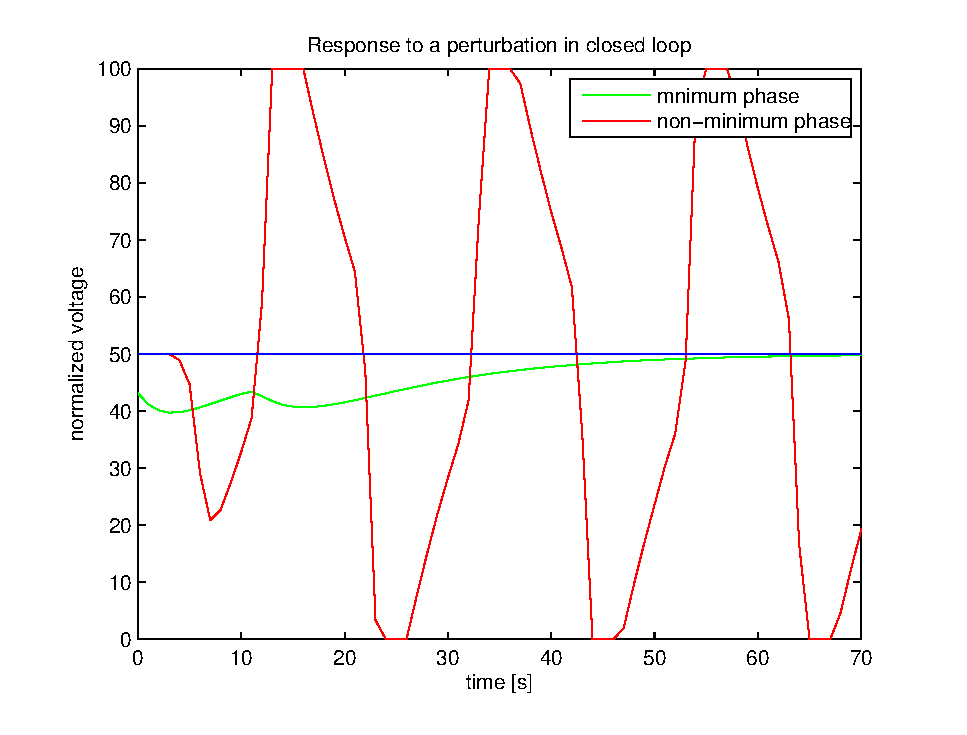
\includegraphics[scale=0.9]{img/pert-rejection-closed-loop.eps}
	\caption{Comparaison des réactions à une perturbation appliquée en
	$t=\SI{10}{s}$ pour un système à non-minimum de phase instable/stable
	et un système à minimum de phase.}
	\label{fig:pert-rej}
\end{figure}

\section{Setpoint tracking}
\begin{figure}[ht]
	\centering
	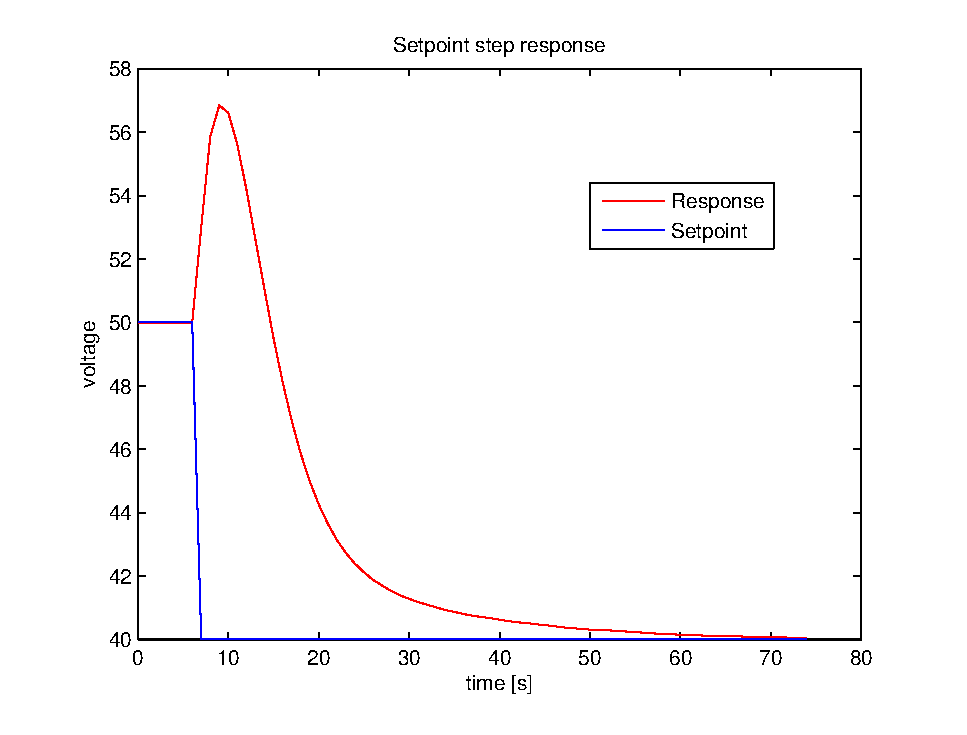
\includegraphics[scale=0.9]{img/setpoint-step-response.eps}
	\caption{Comparaison des réactions à une perturbation appliquée en
	$t=\SI{10}{s}$ pour un système à non-minimum de phase et un système
	à minimum de phase.}
	\label{fig:pert-rej}
\end{figure}



\end{document}